\section{LTS synthesis from high-level MSCs\label{section:inductive-from-hMSC}}

Section \ref{subsection:inductive-synthesis-approach} discussed how system behaviors specified in collections of MSC scenarios can be first generalized as a system LTS, then decomposed as a set of agent LTSs. The QSM technique supports the incremental enrichment of an initial scenario collection through scenario queries. It also takes other models into account, such as goals, so as to preserve multi-view consistency. Behavior generalization, incremental synthesis and multi-view consistency were the three main requirements identified in Section \ref{subsection:inductive-synthesis-requirements}. 

When it is coupled with other synthesis techniques such as goal mining from scenarios\footnote{whose simplest form consists in asking ``why'' questions about negative scenarios.} \cite{Damas:2006}, interactive LTS induction appears really effective; starting from a small initial scenario collection, richer system models can be synthesized through a few iterations only. Chapters~\ref{chapter:evaluation} and \ref{chapter:tool-support} will illustrate this claim through evaluations and discussion of tool support.

For non-toy systems, however, large scenario collections might become unmanageable. In particular, the consistency of the collection might be difficult to guarantee without costly refactoring of scenarios. One notable reason is that all scenarios of a collection are required to start in the same system state. This may imply a lot of redundancy in the required input descriptions. Moreover, this constraint may appear arbitrary for end-users who have to draw the scenarios in the first place.

One way to tackle this problem is to use high-level message sequence charts (hMSCs) for structuring scenario descriptions. As detailed in Section \ref{subsection:background-hmsc}, hMSCs are directed graphs where each node refers to a MSC or a finer grained hMSC (see Fig.~\ref{image:train-hmsc}). Scenarios can then be structured by introducing scenario alternatives, sequencing and loops.

A structured form of scenario \emph{helps} specifying a large system with scenarios. It does not \emph{solve} the problem of achieving a complete and consistent view of agent behaviors:
\begin{itemize}
\item capturing all possible interleavings of a distributed system proves difficult with scenarios; a single hMSC is therefore hardly complete in practice;
\item complementary system features are to be specified in complementary models; in addition to multiple system views, specifying system behaviors in multiple hMSCs makes sense.
\end{itemize}

A synthesis technique for merging and generalizing behaviors described in hMSCs appears to be a convenient extension to the synthesis technique described in sections \ref{section:lts-induction-from-mscs} and \ref{section:inductive-mutliview-consistency}. To this end, the LTS synthesis statement is first revisited in Section~\ref{subsection:hmsc-induction-problem-revisited}. Our inductive algorithm is then adapted in Section \ref{subsection:hmsc-induction-algo-adaptation}.

\subsection{Revisiting the LTS synthesis statement\label{subsection:hmsc-induction-problem-revisited}}

Merging multiple hMSCs $H_1,\ldots,H_n$ with respect to trace behaviors amounts to compute the union of their respective languages. This is equivalent to building a new hMSC $H$ reaching the finer-grained $H_1,\ldots,H_n$ from its initial state. Additional positive scenarios $S^+_1,\ldots,S^+_n$, typically coming from scenario queries, may be integrated in a similar way. This is illustrated in Fig.~\ref{figure:multiple-hmscs}.

\begin{figure}\centering
\scalebox{.70}{
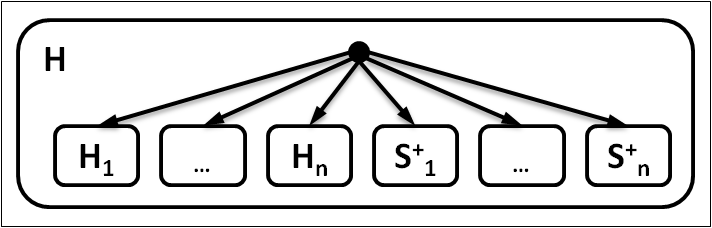
\includegraphics[trim=3mm 3mm 3mm 3mm, clip]{src/4-inductive/images/multiple-hmscs}}
\caption{Merging multiple hMSCs amounts to building a new hMSC reaching finer-grained hMSCs from its initial state.\label{figure:multiple-hmscs}} 
\end{figure}

However, a hMSC only captures positive behavior examples. As explained in previous sections, negative information is needed for avoiding overgeneralization. Negative scenarios, fluents, goals, and the like provide a source of negative knowledge that can be used to constrain the induction process. The algorithmic adaptations introduced in the sequel remain compatible with the constraint mechanism based on equivalence relations on system states. This will be detailed in Section~\ref{subsection:automaton-state-merging}.

We may therefore assume that behaviors are specified through one hMSC only, complemented with a scenario collection. The latter contains negative scenarios and answers to scenario queries. Under these assumptions, the LTS synthesis statement is restated as follows.

\begin{quote}
\underline{Given}~a hMSC $H$ and a scenario collection $Sc = (S^+,S^-)$ consistent with each other, that is,
\begin{align*}
[\mathcal{L}^+(Sc) \cup \mathcal{L}(H)] \cap \mathcal{L}^-(Sc) &= \emptyset
\end{align*}
\underline{Synthesize}~the system as a composition of agent LTSs:
\begin{align*}
System = (Ag_1 \parallel \ldots \parallel Ag_n)
\end{align*}
\underline{Such that}~$H$, $Sc$ and $System$ are consistent with each other.
\end{quote}

The selected hMSC trace semantics is not specified in the formulation above. In other words, the set of behaviors captured by $\mathcal{L}(H)$ has to be decided. Remember the relations between the three hMSC languages discussed in Section \ref{subsection:background-hmsc}: 
\begin{align}
\mathcal{L}_{strong}(H) \subseteq \mathcal{L}_{weak}(H) &\subseteq \mathcal{L}_{arch}(H)
\end{align}

$\mathcal{L}_{strong}(H)$ denotes the set of system behaviors with strong sequential composition of hMSC nodes and total event ordering inside MSCs. It is the simplest model. However, it assumes an implicit synchronization scheme to be used by the agents. The latter is usually not available in real distributed systems. $\mathcal{L}_{arch}(H)$ is the most realistic one for such systems as it captures all possible interleavings of agent behaviors. $\mathcal{L}_{weak}(H)$ is mainly used for explaining and detecting implied scenarios in hMSC specifications \cite{Uchitel:2003}; it is also the hardest to compute.

Making a choice of semantics is required for generalizing behaviors because inductive synthesis takes a set of traces as input. From an algorithmic point of view, however, the three hMSC languages require the same adaptations of the inductive process, as explained in the next sections.

\subsection{Generalizing hMSC behaviors\label{subsection:hmsc-induction-algo-adaptation}}

Remember that learning a regular language $L$ aims at generalizing a positive sample $S_+$ under the control of a negative sample $S_-$ such that the following relation of language inclusions holds:
\begin{align}
S_+~~\subseteq~~L~~\subseteq~~\Sigma^*\setminus S_-
\end{align}

LTS synthesis from a scenario collection $Sc$ reduces to grammar induction because the sets $\mathcal{L}^+(Sc)$ and $\mathcal{L}^-(Sc)$ are valid positive and negative samples, respectively (see Section \ref{subsection:inductive-lts-synthesis-reduction}). In particular, they denote \emph{finite} sets of traces.

When considering the generalization of hMSC behaviors, the sets of positive and negative traces are $\mathcal{L}^+(Sc) \cup \mathcal{L}(H)$ and $\mathcal{L}^-(Sc)$, respectively. The positive set is no longer a sample because $\mathcal{L}(H)$ might contain an infinite number of traces. Therefore, the current problem statement no longer exactly fits the identification-in-the-limit framework introduced in Section \ref{section:inductive-background}. 

From a theoretical point of view, this means that generalizing hMSC behaviors is a different problem than generalizing MSC behaviors; therefore, further study would be needed to re-state the convergence criteria and the notion of characteristic sample in particular. 

From an algorithmic point of view, however, only a few adaptations of RPNI and QSM appear necessary. They are detailed in the next section.

\subsection{The Automaton State Merging algorithm\label{subsection:automaton-state-merging}}

The algorithm for generalizing hMSC behaviors is our Algorithm~\ref{ASM}, called Automaton State Merging (ASM). As sketched below, its overall structure is very similar to QSM in Section~\ref{section:lts-induction-from-mscs}; the interactive feature is omited here as it raises a few issues that we discuss later. QSM itself being an interactive extension to RPNI, Algorithm~\ref{ASM} is very similar to RPNI itself which might appear suprising at first glance.

The main difference between RPNI/QSM on one side and ASM on the other side lies in the \emph{initial automaton} built by \texttt{Initialize}. RPNI and QSM initially convert the input \emph{sample} as a PTA, hence a tree, whereas ASM converts the input \emph{language} of the hMSC as a LTS, hence a graph. 

\begin{algorithm}
{
\vspace{0.2cm}
\KwIn{A high-level MSC $H$ and a scenario collection $Sc = (S_+, S_-)$}
\KwOut{A System LTS, consistent with both $H$ and $Sc$}

$A \leftarrow $ {\tt Initialize($H$, $Sc$)}\\
\While{$(q,q') \leftarrow $ {\tt ChooseStatePair($A$)}}{
$A_{new} \leftarrow$ {\tt Merge$(A,q,q')$}\\
\If{{\tt Consistent$(A_{new}, S_-)$}}{
 $A \leftarrow A_{new}$
}
}
\Return{$A$}}
\vspace{0.2cm}
\caption{\textsc{ASM}, a state-merging algorithm from high-level Message Sequence Charts\label{ASM}}
\end{algorithm}

More precisely, the adaptations required to the different functions of the algorithm are the following:
\begin{description}

\item[Initialize] This function is adapted to return a LTS instead of a PTA. This LTS is built from two sources:
\begin{itemize}
\item On one side, the positive traces from the input hMSC $H$ are captured through a LTS, provided a suitable choice of hMSC semantics. The choice of $\mathcal{L}_{arch}(H)$ appears natural for distributed systems; in that case, the synthesis algorithm from \cite{Uchitel:2003}, introduced in Section \ref{subsection:background-hmsc}, is used to synthesize the LTS from the hMSC.
\item On the other side, the scenario collection is captured through a PTA, as in RPNI and QSM.
\end{itemize}
The standard algorithm for capturing the union of regular languages is then used \cite{Hopcroft:1979} to merge the LTS and the PTA as a single LTS; the latter is returned by \emph{Initialize}.

\item[ChooseStatePair] The main generalization loop in ASM does not fold up a PTA anymore, but successively merges the states of an automaton, which might be any graph\footnote{hence the ``Automaton State Merging'' name.}. In our current ASM implementation, the \emph{ChoosenStatePair} function is slightly adapted to preserve the RPNI search order. ASM pre-computes the natural order among states of the initial LTS solution returned by \emph{Initialize}. A breadth-first search is used; each state is numbered when visited.

\item[Merge] From a specification standpoint, the \emph{Merge} function does not require specific adaptations. This results from the mathematical definition of a quotient automaton (see Definition~\ref{definition:quotient-automaton}). The function takes an automaton and two states to merge as arguments; it returns the quotient automaton resulting from this state merging. 

From an implementation standpoint, the merging-for-determinization process is often implemented under the assumption of a tree invariant property \cite{Lang:1998}. This property states that, when considering two states to be merged, at least one of them is the root of a tree. Such property holds for RPNI and QSM, even when the Blue-Fringe optimization is used. It is a sufficient condition for the determinization process to be finite. 

Even though it is convenient, the tree invariant property is not required \cite{Lambeau:2008}. The main merging loop and the \emph{Merge} function can be implemented without the tree invariant property because the recursive determinization process stops naturally when non determinism is completely reduced. In practice, an implementation of RPNI/QSM may require changing some data structures and associated algorithms to be converted to ASM.

\item[Consistent] This function does not require specific adaptations either; it is the same as in RPNI or QSM (see Section~\ref{QSM:merging}).

\end{description}

Our current ASM implementation does not go beyond: it is not optimized with the Blue-fringe heuristics; it does not have the interactive feature of QSM; it may not be constrained with domain knowledge. Improvements along these three directions are discussed below.

\subsubsection*{Blue-fringe heuristics}

Adding the Blue-Fringe heuristic to ASM would require two main adaptations: 
\begin{itemize}
\item The LTS returned by \emph{Initialize} should be augmented with error states encoding the negative strings captured by negative scenarios in the collection. This requires a slight adaptation of the algorithm for computing the union of regular language; this adaptation is needed to handle the error states of an augmented PTA built from the scenario collection.
\item In a way similar to the \emph{Merge} function, the distinction made by Blue-fringe between red and blue states may be implemented with \emph{ChooseStatePair} relying on assumptions about the initial solution being a PTA (see Section~\ref{BlueFringe}). In that case, another implementation approach might be taken. From a specification standpoint, the characterization of a intermediate automaton in terms of red, blue and white states does not depend on a tree invariant.
\end{itemize}

\subsubsection*{Scenario questions}

The interactive feature of QSM could be adapted and plugged to ASM. It consist in replacing the main ASM loop by the one of QSM (see Algorithm~\ref{QSM} in Section~\ref{section:lts-induction-from-mscs}). In Algorithm~\ref{QSM}, the \texttt{GenerateQuery} function should be adapted as follows:
\begin{description}

\item[GenerateQuery] The generation of scenario queries relies on the tree invariant property mentioned above. When merging a state pair $(q,q')$, a scenario query is built with the shortest trace leading to $q$ concatenated with the suffixes of $q'$. An invariant in QSM is that $q'$ is the root of a tree; this invariant is used to generate finite suffixes for scenario questions (see Section~\ref{QSM:query}).

If the tree invariant property no longer holds, the \texttt{GenerateQuery} function must be extended with a procedure for extracting finite suffixes from $q'$. This does not introduce any technical issues; for example, pre-computing a spanning tree on the initial LTS would associate finite suffixes to each of its state. What forms a ``good'' suffix for convergence and scenario classification by end-users is however an open question. As the adapted algorithm no longer fits in the identification-in-the-limit framework, the notion of a characteristic sample would need to be adapted.

\end{description}

\subsubsection*{Constraints based on domain knowledge}

Even if not supported by our current implementation, the constraint mechanism discussed in Section~\ref{section:inductive-mutliview-consistency} is fully compatible with ASM. Remember that it relies on the partitionning of PTA states according to equivalence relations extracted from domain knowledge. This partitionning can be performed in a similar way on the LTS returned by \texttt{Initialize}. From an algorithmic standpoint, an effective solution actually relies on specific instantiations of the generic LTS decoration algorithm discussed in \cite{Damas:2011} (see Section~\ref{subsection:qsm-constraints-implementation-notes}).
